\chapter{Classifiers}
\label{classifiers}

At the heart of this project's sentiment analysis lie our three classifiers for subjectivity, polarity and emotion. For reasons we shall discuss in their respective chapters, we have elected to take a supervised approach to learning for all three classifiers. As a result, our classifiers' implementations share much in common. In particular, this chapter shall focus on how this commonality can be unified through our \emph{Classifier} class. This project is largely experimental in nature, looking at how we can best adapt, use and develop existing and new ideas for classifying sentiment on Twitter. As a result, we wanted to design a parent \emph{Classifier} class which would best remove the  complexities of correctly assembling and training our classifiers. We wanted a class which would allow us to focus on experimenting with different feature sets and classification techniques, along with providing tools for gathering and comparing our results. The remainder of this chapter shall first outline our core aims for the class, before going on to discuss our approach. After this we will summarise the methods discussed and implemented within our class, before finally evaluating overall performance against our original aims.

\section{Overview}
\label{overview}

As discussed above, our \emph{Classifier} class hopes to unify the overall approach taken to classification across the three classifiers. In doing so it hopes not only to save time by eradicating repetition, but also simplify and encourage experimentation through intelligent design. The three core aims of the class are:

\begin{enumerate}
	\item \emph{Simple feature selection} when initialising a classifier. For example, we might want to initialise a classifier with just \emph{feature one} before initialising another classifier for a performance comparison, with both \emph{feature one} and \emph{feature two}.
	\item \emph{Simple classifier method selection} when initialising a classifier. For example we may want to compare the performance of our classifiers when using a Support Vector Machine against using a Naive Bayes classifier.
	\item \emph{Unified testing} for classifiers in which key machine learning metrics such as accuracy, recall, precision and f-measure are automatically calculated. This will ease in comparing and contrasting results for changes in feature set and classification method.
\end{enumerate}

\section{Preparing the data}
\label{classifiers:preparing_data}

In order to train our classifier, we first need to prepare our \emph{training data} accordingly. This means building a feature set for our training data, according to both the \emph{features} we want to use, and the \emph{label} with which we are looking to classify statuses, as explained in figure \ref{fig:building_feature_set}.

\begin{figure}[h!]
	\caption{Outline for building feature set}
	\label{fig:building_feature_set}
	\centering
		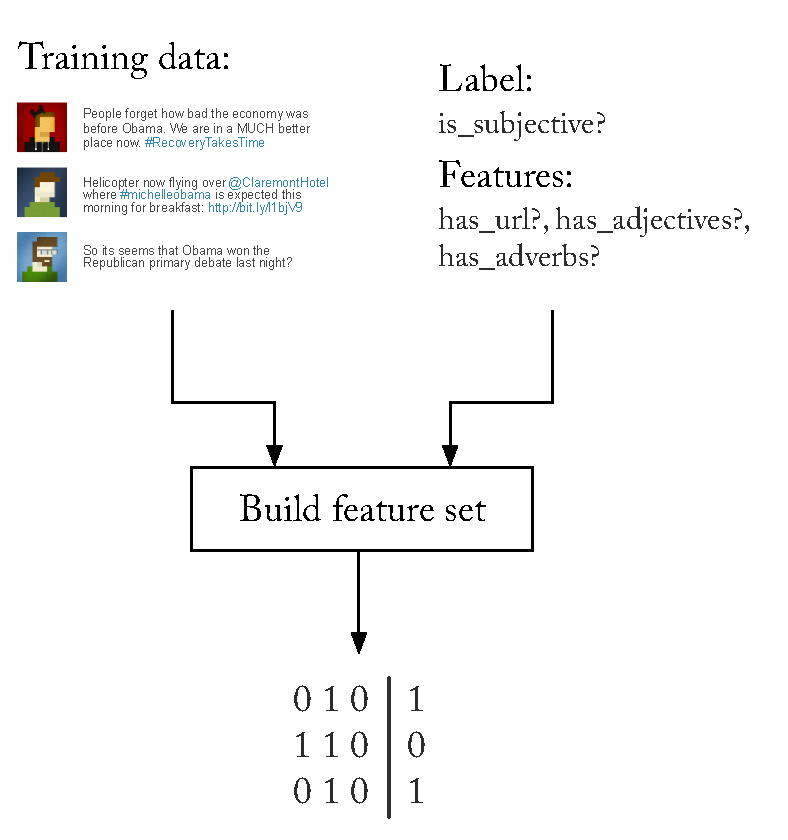
\includegraphics[width=0.6\textwidth]{figures/build_training_data.eps}
\end{figure}

We wanted our approach to this to be as generic as possible, and in doing so made use of Ruby's \texttt{send} method. Every object within Ruby has a \texttt{send} method which accepts a symbol\footnote{\emph{Symbols} are Ruby's approach to efficient \emph{String} usage. In our case, rather than initialising a new \emph{String} object every time we want to refer to a certain method, a symbol is only very initialised once but can be used throughout our code. Essentially a symbol can be used as a low footprint replacement for \emph{Strings}.} and a series of arguments. When called, Ruby will in turn attempt to call the object's method which corresponds to the given symbol, along with any additional arguments. For example \texttt{"Hello, Joe".send(:split, ", ")} is in effect the same as \texttt{"Hello, Joe".split(", ")} and will return \texttt{["Hello", "Joe"]}. It is this we make use of when trying to take a flexible approach to feature choice. It is important to note that all feature methods take a \emph{Status} object and must be implemented as object level methods within any class extending our \emph{Classifier} class. Thus, using the send method, we can initialise our classifier with an array of symbols representing feature methods, before using this array to generically create our training set, as shown in listing \ref{classifiers:status_feature_set}.

\begin{lstlisting}[language=Ruby, caption={Method for building a status' feature set}, label=classifiers:status_feature_set]
# @features = [:feature\_1,..., :feature\_n]
def build_status_feature_set(status)
	return @features.map{|f| self.send(f, status)}
end
\end{lstlisting}

Given a training set, we simply iterate over it, creating a feature set for each training status. This array of feature sets can now be used to train our classifier.

Before we train our classifier, we also need an array containing each of the training statuses' appropriate label, such as their polarity or subjectivity. It is the values of this label which are classifier will be trained to identify, and just as we defined an array of features to build our feature sets, we will instantiate a single \texttt{label} variable to store the label's method symbol, such as \texttt{:is\_subjective?} or \texttt{polarity}. This is built in a similar manner to our feature sets, using the object \texttt{send} method coupled with the \texttt{label} symbol, and is wrapped up in the \texttt{fetch\-\_status\-\_label\-(status)} method.

\section{Training and classifying}

With our training data now prepared in the form of two arrays, one containing feature sets and one containing labels, we can train our classifier. As explored by Pang et al. \cite{Pang:2008wj}, the classification method used can impact the effectiveness of our results. We decided to experiment with both the leading probabilistic and non-probabilistic methods, these being the \emph{Naive Bayes (NB)} classifier and the \emph{Support Vector Machine (SVM)}. 

Rather than building our own SVM and NB classifiers, we elected to use two well established libraries, LIBSVM and AI4R, as discussed in section \ref{background:tools}. As both utilise their own methods and input schemas for training and classification, we implemented an intermediary interface for both the LIBSVM and the AI4R libraries. Both our \emph{NaiveBayes} and \emph{SupportVectorMachine} classes adhere to this interface, and share the same public methods. Effectively this allows us to initialise both our classifiers using the feature sets and labels generated above, as demonstrated in listing \ref{classifiers:build_classifiers}. 

\begin{lstlisting}[language=Ruby, caption={Example initialisation of LIBSVM and AI4R Naive Bayes classifiers through intermediary layer}, label=classifiers:build_classifiers]
feature_sets = training_statuses.map{|s| self.build_status_feature_set s}
labels = training_statuses.map{|s| self.fetch_status_label s}
svm = SupportVectorMachine.new(feature_sets, labels)
nb = NaiveBayes.new(feature_sets, labels)
\end{lstlisting}

Whenever a class extending our \emph{Classifier} class is initialised, an additional parameter is passed in alongside the features and label, denoting whether to use a SVM or NB classification method. A new classification method is initialised as described above, and stored within the \emph{Classifier} object's \texttt{classifier} variable. Once the \emph{NaiveBayes} and \emph{SupportVectorMachine} layers have been initialised and trained, they can be used to classify statuses through their \texttt{classify(feature\_set)} method. When given a feature set, this method will classify it and return the appropriate label. This enables us to again make use of the \texttt{build\-\_status\-\_feature\-\_set\-(status)} method from within our \emph{Classifier} class, rather than having to generate a feature set in the appropriate format for the specified classifier method. In order to better illustrate the chain of command, we have included the \emph{Classifier} class' \texttt{classify(status)} method in listing \ref{classifiers:classify}.

\begin{lstlisting}[language=Ruby, caption={\emph{Classifier} class' classify method}, label=classifiers:classify]
def classify(status)
	feature_set = self.build_status_feature_set status
	# @classifier is either an initialised SupportVectorMachine or
	# NaiveBayes object. This is instantiated when initialising our
	# Classifier object.
	return @classifier.classify(feature_set) 
end
\end{lstlisting}

With unobtrusive support for different feature sets and classification methods now implemented within our \emph{Classifier} class, we can finally look at the approach taken to performance testing.

\section{Testing}

Due to the project's strong element of experimentation, providing a robust framework for evaluating our classifiers was essential. As is common within both machine learning and sentiment analysis, our four chosen measure of performance are \emph{accuracy}, \emph{precision}, \emph{recall} and \emph{f-measure}. These four metrics combine to give a fairly clear portrait of a classifiers strengths and weaknesses. In order to better explain each measure we shall first introduce four terms commonly used within binary classification:

\begin{description}
	\item [True positives] are the set of of correctly classified documents for the positive label. For example in subjectivity classification, this could be taken to be all statuses correctly classified as subjective.
	\item [True negatives] are the set of correctly classified documents for the negative label. For example in subjectivity classification, this could be taken to be all statuses correctly classified as not subjective.
	\item [False positives] are the set of incorrectly classified documents, who have been labelled positive when they are in fact negative.
	\item [False negatives] are the set of incorrectly classified documents, who have been labelled negative when they are in fact positive.
\end{description}

Using these four definitions, we can now go onto better define our performance measures:

\begin{description}
	\item [Accuracy] is used to measure how many documents have been correctly classified across the entire training set.
	\begin{equation}
		accuracy = \frac{| TP \cup TN |}{| TP \cup FP \cup TN \cup FN |}
	\end{equation}
	\item [Precision] is a measure of how accurate our positively labelled data is. This is done by looking at what fraction of positively labelled data is actually positive.
	\begin{equation}
		precision = \frac{| TP |}{| TP \cup FP |}
	\end{equation}
	\item [Recall] is a measure of how much of our positive data is correctly labelled as positive by the classifier. This is done by looking at what fraction of positive data was correctly labelled.
	\begin{equation}
		recall = \frac{| TP |}{| TP \cup FN |}
	\end{equation}
	\item [F-measure] combines the classifiers precision and recall rates to give an overall measure of accuracy.
	\begin{equation}
		F_1 = 2 \cdot \frac{precision \cdot recall}{precision + recall}
	\end{equation}
\end{description}

With the definitions of our measures in place, we now had to introduce a suitable method for calculating them. The first method, \texttt{test(k,statuses)}, performs \emph{k-fold cross validation} across the labelled \emph{statuses} passed in to the method. Effectively k-fold cross validation divides our labelled statuses up into $k$ partitions, before iterating through them, each time using $(k-1)$ partitions as training data, and $1$ partition as testing data. This is repeated $k$ times, and the average measures across each of the folds are taken as the test's overall measures. In order to ensure that training is not biased, we always keep the number of training examples belonging to each label the same.

Although this proved suitable for binary classification, it is not suitable for multi-class classification. Instead for classification with two or more output labels, the \emph{precision}, \emph{recall} and \emph{f-measure} are returned for each potential label. As \emph{accuracy} is already measured across all labels, there was no need for it's results to be calculated for each indiviudal label. The full implementation details for this can be seen in listing \ref{}.

We felt however that for strenuous testing one test was not enough, and instead a \texttt{repeat\_test(k,statuses,n)} method was introduced. This repeats the \texttt{test(k,statuses)} method $n$ times, before returning the average of the measures across those $n$ repetitions.

\section{Class summary}

Before we evaluate the performance of our classifier, we will give a quick overview of the core methods along with a description of their inputs, outputs and purpose.

\begin{centering}
	\begin{longtable}{| l | p{0.16\textwidth} | p{0.16\textwidth} | p{0.4\textwidth} |}
		\hline
		Method & Arguments & Returns & Description \\
		\hline
		\texttt{initialize} & \texttt{features}, \texttt{label}, \texttt{classifier\_method}, \texttt{statuses} & \texttt{none} & Intialisation method for creating new Classifier objects. Will intialize and train either a SVM or NB classifier, with the specified \texttt{features} and \texttt{label}, using the labelled \texttt{statuses} as training data. \\
		\hline
		\texttt{classify} & \texttt{status} & \texttt{label} & The classify method takes a \texttt{status} object, converts it into the appropriate feature set before using the trained classifier method to classify the feature set and return the appropriate \texttt{label}. \\
		\hline
		\texttt{test} & \texttt{k}, \texttt{statuses} & \texttt{accuracy}, \texttt{precision}, \texttt{recall}, \texttt{f-measure} & Given a set of \texttt{statuses}, will split the data into \texttt{k} folds, before testing and training with each. Returns average \texttt{accuracy}, \texttt{precision}, \texttt{recall} and \texttt{f-measure} across the \texttt{k} folds. \\
		\hline
		\texttt{repeat\_test} & \texttt{k}, \texttt{statuses}, \texttt{n} & \texttt{accuracy}, \texttt{precision}, \texttt{recall}, \texttt{f-measure} & Runs \texttt{test(k, statuses)} \texttt{n} times, returning the average \texttt{accuracy}, \texttt{precision}, \texttt{recall} and \texttt{f-measure} across those \texttt{n} repetitions. \\
		\hline
	\end{longtable}
\end{centering}

\section{Evaluation}

The \emph{Classifier} class proved fundamental within this project both as a class and a tool. It has allowed for the remainder of our implementation to focus on innovative feature use and performance, rather than a struggle for consistency across different classifiers. In order to better evaluate the classifier, we shall examine to what extent it met it's original three aims:

\begin{enumerate}
	\item The approach taken to simple feature switching meant that new ideas could be experimented and developed easily, without having to worry about adapting our code elsewhere.
	\item As with feature selection, the class' ability to swap classification methods was simple and effective. It required no additional work throughout the remainder of the project and made evaluation much simpler.
	\item The strong performance testing suite provided a very simple method for meaningfully comparing features and classification methods. This proved vital in understanding how best to approach feature and method selection, along with being fundamental to our evaluation process.
\end{enumerate}

Although no numeric measure can be given to express the class' performance, the fact that it met each of its original aims and the freedom it gave to focus on innovation and testing clearly made it a success.
